\section{引言}
\label{sec:intro}

基准论文通常只报告一张表：模型、准确率、鲁棒性差值、图像依赖得分。医学 VLM 正被越来越多地用于胸片解读~\citep{chen2024chexagent,sellergren2025medgemma,bai2025qwen25vl}，每次新模型发布也都会附带这样一张表。读者由此推断：依赖得分越高，模型越使用图像；退化差值越小，模型越鲁棒；在一个医院验证过的模型，在另一家医院也会有相近表现。上述每一条推断都依赖一个几乎从未声明的前提。在一次跨三个数据集、六个模型、270,324 次调用的评测中，我们发现违反任一前提都会\emph{反转}结论。

\textbf{反转 1（响应性）。}在 PadChest 上，六个模型中有五个的空白对照差异几乎为零：把胸片换成一个均匀灰色方块，89--100\% 的回答逐字节相同。自然解读是``这些模型忽略了外来图像''。但可辩护的解读不同：这些模型对 1,500 张不同的胸片只给出 \textbf{1--20 种不同回答}。没有变化可供解释。限制到 265 例至少含一个疾病标签的研究，仍不能挽救这一解读——五个模型依旧坍缩到 1--8 种回答。依赖是\emph{不可识别}的，而不是零。这一区分很重要：若基准报告``依赖 $\approx 0$''，读者会以为模型对图像退化鲁棒；实际上模型根本没有对任何图像作出响应。

\textbf{反转 2（零模型）。}在 Open-i 上，Qwen3-VL 的空白对照相对真实报告的平均 Jaccard 为 0.091——这看似是一个很强的视觉 grounding 信号，与无图像消融文献报告的效应类似~\citep{anon2026see,anon2026guess}。但每个模型的空白回答都坍缩为一条模板；对 Qwen3-VL 而言，该模板是\emph{``由于缺少图像数据，本研究无法判读。''}正确的零模型不是``与零的相似度''，而是``两份\emph{不同真实}报告之间的相似度''（0.740）。因此，空白对照测量的是\textbf{对图像缺失的检测}，而不是证据提取。Qwen2.5-VL 也有同样混淆（空白 Jaccard 0.576 对真实报告间 0.770）：其空白回答是第二条模板，而它的真实报告有 22.6\% 也是同一模板。没有零模型，排序是任意的；有了零模型，大部分表观信号消失。

\textbf{反转 3（工作点）。}在 NIH 上，重度对比度降低使 InternVL3.5 的合并阳性召回率\emph{提高} 4.69\,\pp{}。单独报告这一数字，会被读作``鲁棒''。但在同一单元中，阳性预测率上升 4.06\,\pp{}，精确率下降 1.38\,\pp{}，假阳性从 1,646 增至 1,905。模型并没有变得更鲁棒；它移动的是工作点。任何只报告召回率或准确率、不报告工作点的鲁棒性基准~\citep{anon2025corruption,anon2026stress} 都可能被这一模式反转，而我们在两个模型家族中都观察到了它。

\textbf{反转 4（契约与输出模式）。}MedGemma-1.5 的图像依赖信号从 4-bit 到 bf16 上升 2.21 倍（0.129 $\rightarrow$ 0.284），读起来像``量化抑制了视觉 grounding''。事实并非如此。同一次切换中，真实图像上的推理通道触发率从 0.13\% 变为 99.07\%，空白图像上 \texttt{no\_finding} 的正向回答从 0\% 变为 100\%。模型切换了\textbf{输出体制}；两组依赖数字不可通约。对照模型 MedGemma-4B 没有发生这种切换（两种精度下标记率均为 0），因此该现象不是``量化''本身，而是``精度诱发的模式切换''。

这四次反转不是彼此孤立的缺陷。它们共享同一结构：一个被报告的数字，其分母、对照或体制从未被建立。我们把这一结构转化为\textbf{四个前提}（第~\ref{sec:preconditions}~节），并在一个满足其余所有控制条件的协议上逐一评测（第~\ref{sec:protocol}~节）。这些检查很便宜——四项审计都可在 CPU 上、对基准本来就已产生的工件运行。

本文有五项贡献：
\begin{enumerate}[leftmargin=1.2em,itemsep=2pt,topsep=2pt]
\item \textbf{一个前提框架}，用于图像依赖、鲁棒性与迁移：响应性、零模型、工作点、契约覆盖。每一项都被操作化为具有明确分母的统计量，并证明省略它会使结论反转。
\item \textbf{一个退化的双轴描述模型}：\emph{可察觉性}与\emph{损伤}可分离，二者的联合分布刻画出\textbf{静默失效象限}。噪声在 MedGemma-1.5 上是极端案例：损伤与分辨率损失相当，可察觉性低两个数量级。第二个推理模型（第~\ref{sec:results-second} 节）复现了可分离性，但没有复现象限归属，从而把``静默失效''定位到监测通道而非退化本身。
\item \textbf{契约依赖性结果}：同一模型、同一张空白图像，在一种契约下给出 1,506/1,506 条模式合规的``自信正常''回答，在另一种契约下给出 1,506/1,506 次弃答；CheXagent 有 79\% 的标签槽位为 \texttt{not\_mentioned}，这改变了每个选择性指标的分母。
\item \textbf{四项受控复现实验}（第~\ref{sec:results-round2} 节）：监督基线宏 AUROC 0.733 对六个 VLM 的 0.50--0.63，且同一 CNN 在 19 格网格上以固定 0.5 规则复现了对比度诱发的工作点移动；第二个医学模型上的五套 schema 扫描与 Qwen3-VL 上的跨家族扫描；改写对照（$\kappa$ 0.62--0.64）；以及第二个推理模型，其 89.0\%（8,192 token 抽样后 89.2\%）的可用答案率使\emph{覆盖率}本身成为随损伤变化的量。
\item \textbf{一项具有明确含义的负结果}：复合风险信号只使发现级错误\emph{排序}发生边际变化，在 5\% 风险预算下最多覆盖 9.3\% 的发现；选择性可信框架应作为``未获验证''报告，而不是作为解决方案。
\end{enumerate}

我们刻意不宣称新的 state of the art。这些检查单独看并不新颖：输出多样性、无图像消融、精确率--召回率并列报告、弃答核算都已在既有工作中出现。本文的贡献在于把它们定义为面向同一目标量的\emph{识别条件}，用实证表明省略任一条都会反转结论，并发布一套其他人可以在自己的预测结果上运行的审计流程。本文的主张关于测量：该文献中若干被广泛报告的量，在现行报告惯例下并不可识别。图~\ref{fig:reversals} 汇总了四次反转。

\begin{figure}[t]
\centering
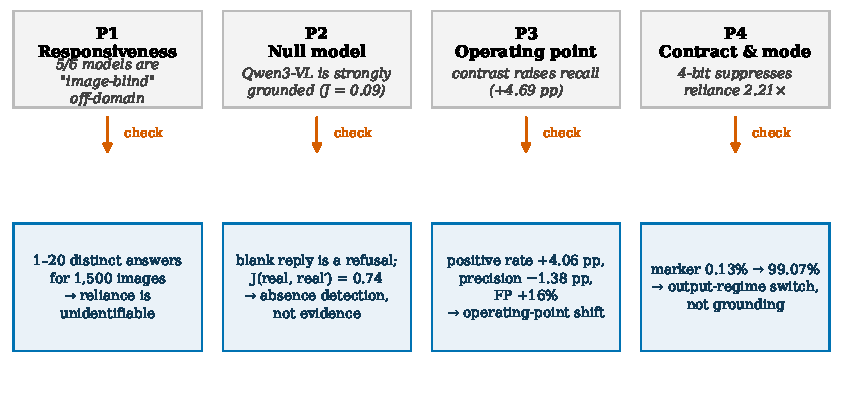
\includegraphics[width=\textwidth]{figures/fig01_four_reversals.pdf}
\caption{四个前提及其所防止的四次反转。上排是仅凭被报告统计量会得到的结论；下排是检查之后应得的结论。}
\label{fig:reversals}
\end{figure}
